\documentclass[runningheads]{llncs}
\usepackage[T1]{fontenc}
\usepackage{graphicx}
\usepackage{subcaption}
\usepackage[UTF8]{ctex}

\usepackage{changes}  % 使用changes宏包
% \usepackage[final]{changes} % 禁用修订,输出最终修订完成的版本
% \usepackage[commandnameprefix=always, defaultcolor=red]{changes}  % 使用changes宏包
\definechangesauthor[name={zheliku}, color=blue]{zheliku} % 修订作者

\bibliographystyle{splncs04}

\AtBeginDocument{%
  \providecommand\BibTeX{{%
    Bib\TeX}}}

\begin{document}

\title{VRTI:为沉浸式物理学习提供真实触觉反馈与手部操作}

% \author{Hailin Ji\inst{1} \and 
% % \orcidID{0009-0002-3512-6730} 
% Yihang Li\inst{1} \and 
% Yiran Zhang\inst{1} \and 
% Hongwen Zhang\inst{1} \and 
% Xiaoyan Hu\inst{1} \and 
% Yanhong Luo\inst{2}}
 
% \authorrunning{H. Ji et al.}

% \institute{Beijing Normal University, Beijing, China \and
% Northwest Minzu University, Beijing, China}

\author{匿名作者}

\maketitle

\begin{abstract}
随着手势追踪技术的成熟,基于VR的沉浸式学习环境支持与虚拟对象的自然手势交互(GI),提供直观的教育体验。然而,GI中触觉反馈的缺失削弱了沉浸感。
\added[id=zheliku]{
  本文提出虚拟-现实孪生交互(VRTI),通过同步虚拟交互对象(VIO)与真实交互对象(RIO)为手势提供动态触觉反馈。核心创新包括:
  1) \textbf{道具触觉动态化}:实时传感网络通过时空同步将物理道具的静态属性转化为动态反馈。
  2) \textbf{手势-道具一致性模型}:实现视觉-触觉同步交互,支持手部操作期间的交互校准。
  应用于高中动量守恒实验,三种VR孪生体(拉杆/按钮/旋钮)支持抓握、按压和捏取操作。对照试验(VRTI: N=32 vs GI: N=32)表明VRTI:
  1) 显著提升学习动机(p<0.001)和沉浸感(p<0.001)。
  2) 降低外部认知负荷(p<0.001, |r|=0.625)。
  3) 提高实验理解度(p=0.05)和知识应用能力(p=0.005)。
}

\keywords{虚拟-现实孪生交互 \and 虚拟现实 \and 触觉反馈 \and 物理教具 \and 沉浸式物理学习 \and 手势交互}
\end{abstract}

\section{引言}
随着VR技术的快速发展,沉浸式学习环境已成为研究热点并广泛应用于教育、娱乐和医疗等领域 \cite{luo2020dream,yeung2021virtual}。将沉浸式学习环境引入物理实验教学可解决传统方法面临的难点,如理解困难、成本高昂、操作繁琐和资源有限等 \cite{yang2007impact,abu2018design}。通过革新传统教学模式,沉浸式学习环境创造更具交互性和吸引力的体验,激发学生学习兴趣和动机。例如,Dalgarno \& Lee的研究表明沉浸式学习环境显著提升学生理解复杂概念的能力并促进深度学习 \cite{dalgarno2010learning}。Campos等人在大学物理课程中使用沉浸式环境教授矢量概念,学生可在3D网格中操作矢量、识别角度分量并测量模长,结果凸显了该方法在培养抽象概念化和操作技能方面的潜力 \cite{campos2022impact}。

沉浸式学习环境通过视听手段模拟实验现象,降低设备要求并提高实验灵活性,为物理实验教学开辟新可能。然而,以视觉为主导的交互缺乏真实物理实验中的触觉反馈,使传统沉浸式环境难以提供真实的物理操作体验 \cite{giri2021application}。学习者在虚拟环境中仅能观察物理现象,无法通过触觉反馈感知真实的力作用,导致学习体验不完整。物理实验不仅是现象观察,更涉及对力与物体相互作用的直接感知。因此,在沉浸式物理学习环境中集成触觉反馈至关重要。通过触觉反馈,学生可感知虚拟环境中物体的重量、阻力和弹性,获得更直观的操作体验,深化对物理概念和定律的理解 \cite{minaker2016handson}。然而传统触觉设备通常仅提供基础力反馈,且可能限制学习者的交互动作,难以满足物理实验中复杂手部操作的需求 \cite{bonfert2023challenges}。例如真实物理实验中,手部操作包含抓握、按压、捏取、旋转和拖拽等多种动作,这些操作不仅需要精确控制手部运动,还需感知和调节力的大小、方向和作用点,这对实验成功至关重要。现有触觉设备无法准确模拟这些手部操作,导致虚拟实验与真实操作体验存在显著差距。

综上所述,本研究的主要贡献如下:

\added[id=zheliku]{
  第一,我们提出虚拟-现实孪生交互(VRTI),该框架通过引入物理对象与虚拟对象的实时时空同步,扩展了被动触觉代理技术。与现有静态道具不同,VRTI通过传感器-执行器同步实现动态力反馈,同时在复杂操作中保持精确的虚实对齐。
}

第二,我们提出VRTI的虚实对齐方法以解决手部与VR孪生体的穿透问题。手势追踪中的位置和方向误差常导致虚拟手与VIO发生穿透。我们的方法通过手势预测优化解决视触觉错位问题,在保持交互真实性的同时消除穿透现象。

最后,我们通过教学实验验证VRTI的优势。与XXX大学物理系教授及研究人员合作,设计了符合高中物理课程的动量守恒实验。VRTI($N=32$)与GI($N=32$)的对照研究表明:
\begin{enumerate}
  \item 未显著增加认知负荷($p = 0.602$)
  \item 显著提升学习动机($p < 0.001$)和沉浸感($p < 0.001$)
  \item 比单独使用GI更有效提升实验内容理解度($p = 0.05$)和知识应用能力($p = 0.005$)
\end{enumerate}

\section{相关工作}
\subsection{VR学习理论}
研究表明在教育场景应用沉浸式VR可提升学生学习体验并增进知识理解 \cite{freina2015literature}。理解并应用VR学习理论有助于教育者设计更优质的学习材料和评估工具,发展更有效的教学方法 \cite{matovu2023immersive}。因此,学习理论在VR学习体验设计中的应用日益重要 \cite{marougkas2023virtual}。常见VR学习理论包括认知负荷理论、ARCS动机模型和沉浸理论。

认知负荷理论由John Sweller于1988年提出,是理解学习与认知的框架 \cite{sweller1988cognitive}。该理论将认知负荷分为三类:内部认知负荷(intrinsic)、外部认知负荷(extraneous)和关联认知负荷(germane)。内部认知负荷与学习材料固有复杂性相关且不可避免,取决于任务复杂度和学习者先验知识;外部认知负荷由教学设计中与学习目标无关的干扰因素引起;关联认知负荷涉及学习过程中认知结构的构建与自动化,促进理解和记忆。主流观点认为:分解复杂任务可降低内部认知负荷;消除冗余信息可减少外部认知负荷;练习与重复则通过帮助学习者构建和自动化图式来增加关联认知负荷 \cite{baceviciute2022investigating}。

ARCS动机模型由John M. Keller于1987年提出,是教育领域广泛应用的动机框架 \cite{keller1987development}。该模型指出学习动机的激发与维持依赖于四个核心要素:注意力(Attention)、相关性(Relevance)、信心(Confidence)和满意度(Satisfaction)。通过吸引学习者兴趣(注意)、确保学习内容相关性(相关)、增强学习者信心(信心)和提供成就感(满足),ARCS模型帮助教育者设计更具吸引力和成效的教学策略。该模型不仅适用于传统课堂,也广泛应用于VR教育等现代教育技术中,成为提升学习动机的重要理论工具。

沉浸感指用户交互过程中在虚拟环境中产生的"身临其境"感。Sherman等人将沉浸分为物理/感官沉浸和心理沉浸 \cite{sherman2003understanding}。在虚拟环境中,用户通过视觉、听觉和触觉等感官获取信息,经感知系统处理实现自由导航和虚拟对象操作,达成物理沉浸。心理沉浸指深度投入虚拟环境的状态。两类沉浸均显著影响用户体验。自由导航、第一人称视角、真实感和交互性等特性有助于提升学习者的沉浸感 \cite{regenbrecht2002real,mikropoulos2006presence},其中交互性尤为关键 \cite{schubert2001experience}。

除上述理论外,新理论视角近年也受研究者关注。Ryan R M等人提出的自我决定理论(SDT)强调学习过程中的自主性、能力感和关联性。VR技术通过提供沉浸式交互学习环境,更好地满足这些心理需求,从而提升学生学习动机和效果 \cite{ryan2024self}。Liu J等人探究了VR学习环境自主性与学习者特征如何共同影响学习效果和认知负荷,结果表明单一因素变化未必改变结果,因其常由双因素交互作用决定 \cite{liu2024autonomy}。Lui A L C等人综述了基于学习理论的VR教育研究,提出六项设计原则以促进传统课堂教育向VR转型,为未来教育者提供理论指导 \cite{lui2023theory}。随着技术进步与教育需求演变,VR学习理论与实践将持续发展完善。

\subsection{沉浸式物理学习}
随着VR技术进步,其在沉浸式物理学习中的应用日益广泛。例如Georgiou等人在狭义相对论理论学习中引入沉浸式VR,让学生以第一视角体验相关物理现象,提升学习效率和动机 \cite{georgiou2021learning}。Campos等人在大学物理课程中使用沉浸式环境教授矢量概念,学生可在3D网格中操作矢量、识别分量与角度并测量长度,该方法展现出培养抽象概念化和操作技能的潜力 \cite{campos2022impact}。此外,AR技术通过将虚拟对象叠加至真实环境增强用户体验,使通常不可见的实验要素可视化,帮助学生深入理解科学原理 \cite{pegrum2021augmented,prahani2022trend}。例如研究者将力学中的力矢量和电磁学中的电势分布在3D空间中可视化,促进学生理解复杂物理现象 \cite{al2020effectiveness,teichrew2020augmented,ismail2019enhancing,boettcher2021using}。

尽管沉浸式物理学习环境日益受到关注,大多数研究和实践仍聚焦于使用视觉反馈传递信息,忽视其他感官交互。作为人体与物理世界的直接连接,触觉提供关于形状、纹理、温度和重量的即时信息,在人类感知体验中扮演重要角色 \cite{zhang2023active}。现有研究表明,融入触觉反馈可显著增强虚拟学习环境效果。例如Shen Yang等人将触觉反馈技术引入K-12物理实验场景设计,通过准实验评估其在沉浸式学习中的应用。结果表明在VR沉浸式学习中使用触觉反馈显著提升学习者的真实感和交互效率,但对知识获取影响不显著 \cite{shen2023research}。Johnson-Glenberg等人证明,在STEM教育的VR环境中,添加触觉信息显著降低认知负荷并增强学生对知识的理解和保持,尤其当学生具备先验知识时效果更佳 \cite{johnson2023embodied}。教育中的具身认知理论表明,通过身体感知和操作,学习者可将具体经验转化为抽象知识,在心理层面重建和模拟实际体验 \cite{varela2017embodied}。触觉技术通过模拟真实世界交互,使虚拟实验更具吸引力和真实感,有效提升学习效率,在帮助学生理解复杂概念方面发挥不可或缺的作用 \cite{shapiro2019embodied}。因此在沉浸式物理学习环境中集成触觉交互,探索触觉在沉浸式物理学习中的最优应用模式应成为未来研究趋势和重点。

当前支持触觉反馈的沉浸式物理学习环境主要分为两类:触觉反馈设备和基于AR的系统。触觉反馈设备通过电机、液压或气动系统产生可控物理力作用于用户手部或身体,模拟真实触觉反馈(如拉力、推力和阻力)。沉浸式物理学习环境中常见的触觉反馈设备包括触觉反馈操纵杆/机械臂(如PHANTOM系列)、触觉手套(如HaptX手套)和振动设备(如VR控制器)。例如Qi K等人设计了液体容器实验交互环境,使用Novint Falcon触觉设备探究触觉与视觉反馈对理解浮力相关基础物理概念的影响 \cite{qi2020impact}。Acevedo P等人创建电磁场可视化环境,使用Oculus Quest VR控制器提供振动反馈,研究虚拟现实环境和触觉反馈对学生电磁学感知和理解的影响 \cite{acevedo2022effects}。另一方面,AR技术将虚拟信息叠加至真实世界,通过可触摸物理对象(如模拟工具或模型)提供沉浸式触觉反馈。例如Knierim P等人使用实物副本替代实验室实验中的物理组件,通过AR提供触觉反馈并可视化工作流程,比较用户在设置时间、工作负荷、测量质量和学习任务概念理解方面的表现 \cite{knierim2020tangibility}。Liu Q等人设计开发基于AR的中学物理磁场概念移动模拟工具,探究其对学生的知识提升和认知负荷影响 \cite{liu2021effects}。

\subsection{触觉交互}
人类触觉感知包含动觉和皮肤反馈。动觉反馈指由皮肤、关节、骨骼肌和肌腱中的感受器介导的身体位置和运动感觉;皮肤反馈则与皮肤下低阈值机械感受器检测的刺激相关,使人能通过触觉感知自然或合成的机械环境 \cite{hayward2004haptic}。随着VR技术持续发展,仅靠头戴设备提供的视觉信息输入已无法满足交互需求,触觉反馈在VR环境中的重要性日益凸显。通过引入触觉技术,用户在与物理或虚拟环境交互时获得触觉反馈 \cite{sreelakshmi2017haptic},这不仅弥补了视觉信息的局限,更为用户提供更丰富真实的感知体验,使其直观理解虚拟环境中的物体和交互。

近十年来,触觉技术进步带动相关设备显著增长。触觉设备作为触觉技术的载体,使用户能与计算机生成的虚拟环境进行直观沉浸的交互 \cite{sreelakshmi2017haptic},主要分为三类:固定式设备(桌面设备)、手持式设备和可穿戴设备 \cite{adilkhanov2022haptic}。固定式设备因尺寸或功能特性无法穿戴于用户身体特定部位,工作空间有限。可进一步分为可抓握设备 \cite{adel2018rendering,zarate2020contact,feick2023voxelhap} 和可触摸设备 \cite{adilkhanov2020vibero,goetz2020patch}。手持式设备可手持携带,相比固定式设备具有便携性、较少移动限制和更大工作空间,但不支持完全自由移动。根据驱动类型,手持设备可分为直接驱动设备 \cite{sakr2020haptic,chen2019haptivec} 和间接驱动设备 \cite{kovacs2020haptic}。直接驱动设备通过手柄和执行器直接作用于用户手部,间接驱动设备则通过改变重心提供不同触觉提示。可穿戴设备根据佩戴部位分为触觉手套 \cite{ozioko2022smart}、指戴设备 \cite{chinello2019modular,preechayasomboon2021haplets} 和臂戴设备 \cite{zhao2020wearable,pezent2022explorations}。

与传统触觉设备不同,基于手部的触觉交互聚焦虚拟手模型与触觉渲染的集成。相关研究包括虚拟手的几何与物理建模、基于虚拟手的碰撞检测与力计算,以及动觉与触觉渲染 \cite{tong2023survey}。两大挑战持续存在:(a) 在VR体验中使用真实物体模拟触觉反馈;(b) 实现真实/虚拟手部与物体的空间一致性以实现无缝交互(本研究称为虚实对齐)。André Zenner等人证明,动态硬件调整结合基于软件的视觉补偿可显著提升触觉反馈的真实感和鲁棒性,但此类方法仍处于早期阶段 \cite{zenner2021combining}。近年来该研究方向日益受到关注。例如M. Salvato等人使用手势追踪时间序列和虚拟对象几何预测用户何时接触虚拟对象,改进混合现实中的触觉反馈 \cite{salvato2022predicting}。H. Barreiro等人提出新型粒子基粘塑性交互模型和基于优化的超声波渲染算法,结合空气触觉渲染技术模拟类粘土材料交互并提供高真实感触觉反馈 \cite{barreiro2021natural}。Salagean A等人将超声波空中触觉技术应用于VR环境,参与者观看虚拟手被羽毛抚摸时同时在手掌无毛皮肤和手背有毛皮肤接收刺激。结果表明手掌超声波刺激更强烈 \cite{salagean2022virtual}。

\section{方法}
\added[id=zheliku]{
  VR孪生体是基本交互单元,包含物理世界中的真实交互对象(RIO)及其在虚拟环境中的对应虚拟交互对象(VIO)。VIO提供视觉反馈,RIO提供触觉反馈。\deleted{关键在于,}VR孪生体支持用户通过自然手势交互而无需额外学习成本。用户在虚拟交互过程中感知真实触觉反馈,复现操作真实物体的体验。
}

\subsection{数据同步}
VR孪生体的VIO同步其对应RIO的状态(如位置、角度)。二者间的数据通信通过实时传感技术实现。三个VR孪生体均配备特定传感器采集RIO物理属性,经滤波后通过Arduino传输至VIO实现实时更新。

\subsubsection{传感方案}
每个RIO配备应用专用传感器以捕获其物理状态和用户输入。关键\replaced{步骤}{考量}包括:
\begin{enumerate}
  \item 传感器\replaced{选择}{选型}:基于交互模态(如线性位移、旋转运动、压力施加)集成合适传感器(如拉力/称重传感器、加速度计、陀螺仪、压力传感器、旋转编码器、电位器)
  \item 性能规格:传感器特性包括工作频率、量程、分辨率和精度,需根据交互的保真度与动态特性定制。常见参数含采样率(如50-100 Hz)、力量程(如0-20 $N$)、位移/角度分辨率(如0.01 $m/s^2$, 0.5$^\circ$)和压力分辨率(如0.01 $N$)
\end{enumerate}

\subsubsection{数据通信}
鲁棒的通信架构确保RIO与主机系统(如运行VR环境的PC)间的低延迟数据传输:
\begin{enumerate}
  \item 硬件平台:微控制器(如Arduino UNO)作为接口采集原始传感器数据。精密模拟测量采用信号调理模块(如HX711用于高增益放大和24位ADC)
  \item 系统架构:分布式架构具优势。每个RIO(或传感器组)连接独立微控制器实现并行数据采集。微控制器通过独立串行链路(如USB虚拟COM端口)与主机通信
  \item 主机端处理:主机系统实现多端口通信以并行监控所有RIO数据流。数据包通过预定义标识符(设备ID、传感器类型)解析并结构化,供后续处理使用
\end{enumerate}

\subsubsection{数据处理}
原始传感器数据经处理流程提升信号质量、归一化输入并导出有效交互状态:
\begin{enumerate}
  \item \texttt{\added{输入}降噪}:卡尔曼滤波应用于原始数据,通过最优结合预测和含噪测量估计真实系统状态,显著降低环境和传感器噪声影响
  \item \texttt{\deleted{输入}归一化}:传感器读数相对于预定义操作限值归一化至统一范围\deleted{(如}[0,1]\deleted{)}。下限通常对应RIO初始/静止状态,上限通过经验确定(如重复用户试验捕获预期最大输入值)或基于传感器规格
  \item \texttt{状态检测与平滑}:处理/归一化数据($x_t$)用于确定交互状态和平滑过渡:
  \begin{enumerate}
    \item 阈值法:使用经验阈值检测状态变化(如 $x_t > 0.05$)
    \item 变化检测:显著变化($\Delta x_t >$ 阈值)指示状态转换
    \item 插值法:对$x_t$应用线性插值\deleted{等技术}确保VIO状态(位置、旋转)在虚拟环境中的平滑更新
  \end{enumerate}
\end{enumerate}

\subsection{虚实对齐}
虚实对齐确保VIO与其RIO对应物间的精确空间对应和一致交互行为。这对提供真实同步的视觉与触觉反馈至关重要,从而最大化用户沉浸感和交互真实度。

\subsubsection{空间对齐}
RIO以固定空间关系安装(通常在稳定平台上),建立可靠物理参考系。虚拟场景通过定义虚拟单位(如Unity单位)与现实单位(如米)的比例尺构建。VIO在虚拟环境中缩放定位,精确匹配RIO在物理参考系中的相对位置和方向。处理后的RIO传感器数据($x_t$)持续映射至VIO状态控制:
\begin{enumerate}
  \item 线性交互中,$x_t$驱动定义轴上的位移(如 位置 = $x_t \times$ 最大位移)
  \item 角度交互中,$x_t$直接控制旋转
  \item 二元或范围状态(如按下/释放)中,$x_t$在定义状态间插值(如 高度 = 最大高度 - (最大高度 - 最小高度) $\times x_t$)
\end{enumerate}

\subsubsection{交互校准}
实现鲁棒交互需减轻手势追踪固有不准确性,该问题可导致虚拟手穿透VIO或若应用模拟物理则产生非真实物体运动。我们的解决方案采用\replaced{以下三个步骤}{三管齐下方法}:

\paragraph{VIO\deleted{运动}独立性} VIO核心运动\added{属性}(位置、旋转)仅由RIO传感器数据驱动。在物理引擎中赋予VIO无限质量,确保其不受意外虚拟手碰撞影响,防止非自然抖动或位移。

\paragraph{\deleted{手势参数化与}预定义\added{交互库}} \deleted{手部姿态特征(关节位置、手指长度、弯曲角度)被参数化。}为每类VIO预定义交互专用标准手势,优化匹配VIO几何形状和预期操作方法。例如圆柱形物体采用半闭合抓握姿势,按钮按压采用伸展手指姿势。

\paragraph{基于手势预测的动态碰撞\deleted{处理}}:
\begin{enumerate}
  \item 交互触发区:以用户虚拟手掌为中心的球形边界体积定义潜在交互启动的邻近区域(图\ref{fig:bounding-volume})
  \item 手部碰撞模型:简化球体树模型近似虚拟手碰撞几何(如关键关节和手掌处的球体)(图\ref{fig:sphere-tree-model})

  \begin{figure}
    \centering
    \begin{subfigure}{0.4\linewidth}
      \centering
      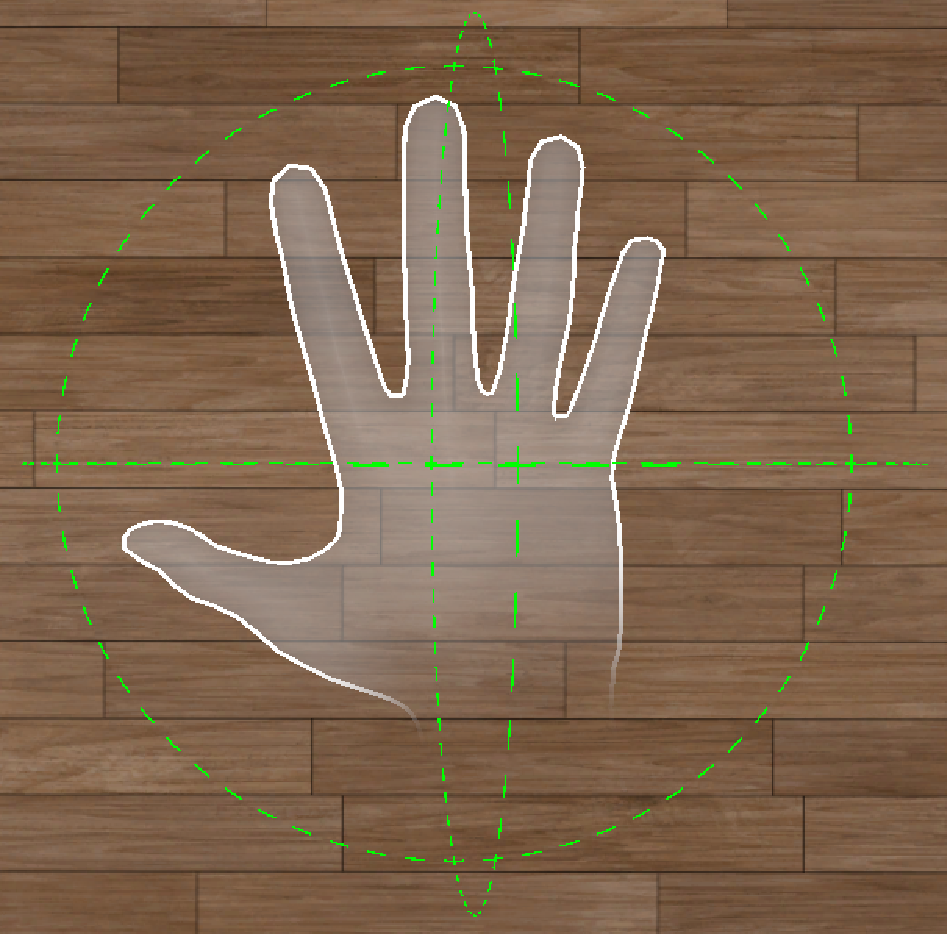
\includegraphics[width=\linewidth]{image/bounding-volume.pdf}
      \caption{}
      \label{fig:bounding-volume}
    \end{subfigure}
    % \hfill
    \begin{subfigure}{0.4\linewidth}
      \centering
      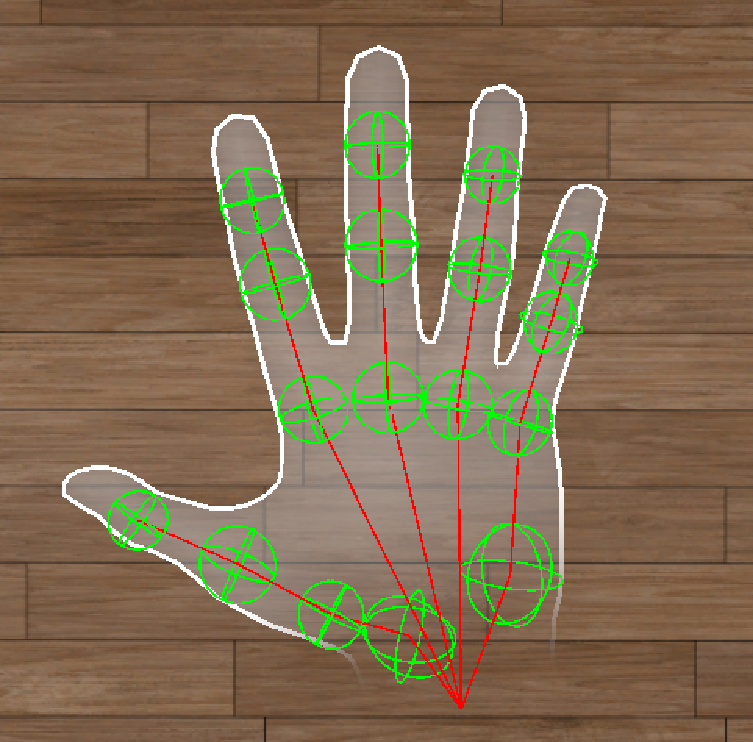
\includegraphics[width=\linewidth]{image/sphere-tree-model.pdf}
      \caption{}
      \label{fig:sphere-tree-model}
    \end{subfigure}
    \caption{虚拟手边界体积与球体树模型。(\subref{fig:bounding-volume})球形边界体积,(\subref{fig:sphere-tree-model})球体树模型}
    \label{fig:bounding-volume-and-sphere-tree-model}
  \end{figure}

  \item 基于状态的碰撞策略:
    \begin{enumerate}
      \item 交互状态:当手部进入触发区且用户追踪手势充分匹配VIO预定义交互手势时,系统启动交互:
      \begin{enumerate}
        \item 虚拟手平滑插值至预设标准姿势以最小化视觉穿透
        \item 禁用手部球体树与VIO的物理碰撞,避免交互手势激活时的穿透伪影
      \end{enumerate}

      \item 非交互状态:在触发区外或无匹配手势时:
      \begin{enumerate}
        \item 启用手部球体树的物理碰撞
        \item 防止虚拟手穿透VIO
        \item 因VIO无限质量,碰撞仅约束手部位置而不引起非真实VIO运动
      \end{enumerate}
  \end{enumerate}
\end{enumerate}

\section{VRTI设计}
\added[id=zheliku]{
  VRTI为需要同步触觉真实性、操作安全性和视觉可扩展性的场景建立闭环交互系统\replaced{,}{。}适用于以下三类交互场景:
}
\begin{enumerate}
  \item \texttt{高风险技能训练领域}(如工业设备维护、医疗手术),RIO保留本体感觉运动链(如扭矩传递、组织穿刺阻力),VIO叠加危险场景可视化和操作指导以降低实操风险
  \item \texttt{复杂系统认知增强}(如科学实验教学、机械原理演示),利用RIO实现物理约束交互(如弹簧振子动力学、化学反应进程),VIO生成多维动态数据表征(如力矢量分解、分子结构演化)以建立多模态认知闭环
  \item \texttt{跨空间协作环境}(如远程设备维护、分布式原型设计),利用RIO同步本地操作参数(如工具扭矩、界面按压深度),VIO构建共享数字孪生体,通过双向触觉-视觉反馈实现协同决策
\end{enumerate}

\subsection{实验场景}
\added[id=zheliku]{
  与XXX大学物理系XXX教授团队合作,\replaced{选择}{确定}实验内容为动量守恒定律验证。选择该\added{物理}实验\replaced{进行设计的原因如下}{基于以下原因}:
}
\begin{enumerate}
    \item 需同时感知力(弹簧)、时间(轨迹)和系统状态(质量比)
    \item 现象涉及不连续状态变化(碰撞),难以用静态道具模拟
    \item 展示可迁移至其他领域的核心物理原理
\end{enumerate}

实验装置由弹簧连接的A、B两滑块组成。学生通过向后拉动B滑块赋予其初速度,使系统在弹簧作用下做周期性运动。实验中学生通过面板可视化数据研究系统运动过程,验证动量守恒定律。具体实验场景如图\ref{fig:experiment-scenario}所示。

\begin{figure}
  \centering
  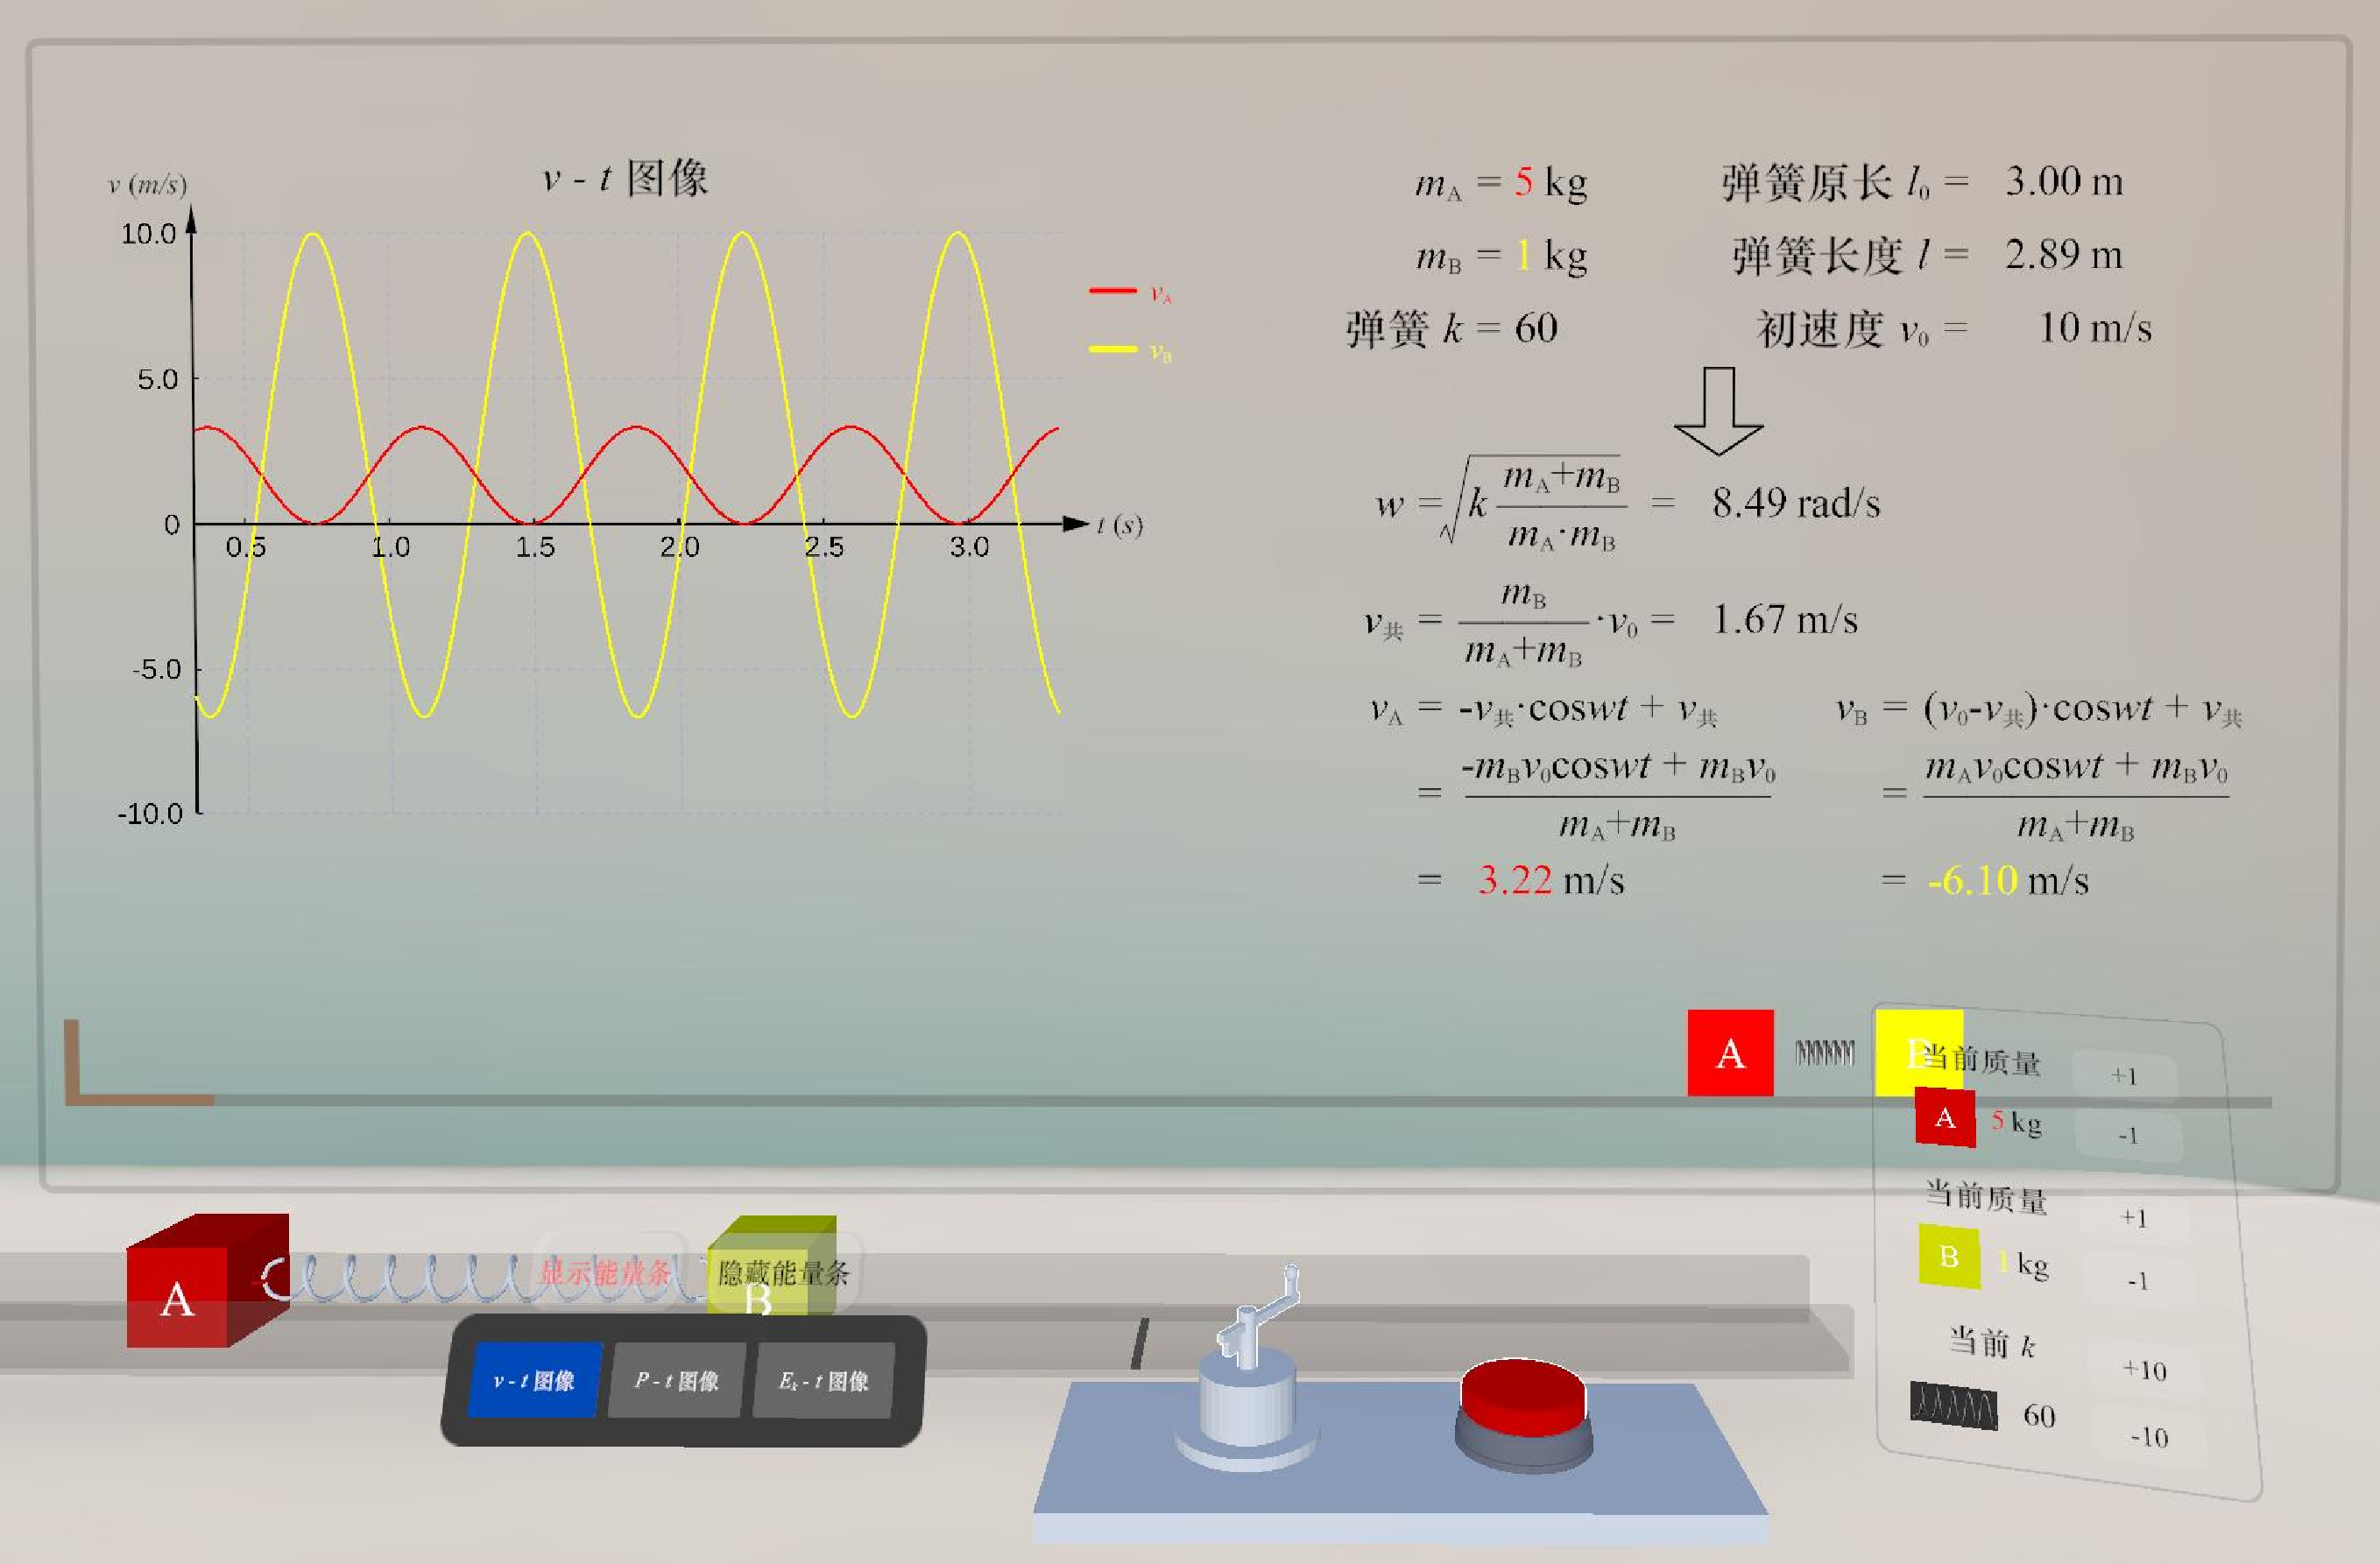
\includegraphics[width=\linewidth]{image/experiment-scenario.pdf}
  \caption{动量守恒实验场景}
  \label{fig:experiment-scenario}
\end{figure}

进入实验场景后,学生首先用食指点击右侧参数设置面板按钮配置实验参数(含两滑块质量和弹簧劲度系数)。随后将B滑块向右拉动至适当力度释放,"发射"B滑块并观察系统运动。接着旋转旋钮调整运动过程时间线(顺时针前进/逆时针后退),探索可视化面板图像特征和物理量关系。最后当系统到达终点位置时按下按钮重置系统并重新配置参数继续探索。

可视化面板左侧提供三图:(1)$v$-$t$图,(2)$P$-$t$图,(3)$E_k$-$t$图,直观显示相应物理量变化。右侧展示对应物理量计算公式,呈现其计算过程。图为按钮交互切换,满足实验教学需求。

\subsection{虚拟-现实孪生体}
基于动量守恒定律验证实验设计,VR孪生体实现包括拉杆、按钮和旋钮。图\ref{fig:structural-diagram}展示各部件结构设计。三者RIO与VIO均源自同一3D模型:RIO通过3D打印获得,VIO通过模型导入Unity创建。因用户视觉反馈直接由VIO提供,VIO在虚拟环境中着色渲染,RIO则保持未着色状态。

\begin{figure*}[t]
  \centering
  \includegraphics[width=1\textwidth]{image/Structural-Diagram.pdf}
  \caption{三种VR孪生体结构图}
  \label{fig:structural-diagram}
\end{figure*}

\begin{figure*}[t]
  \centering
  \includegraphics[width=1\textwidth]{image/Interaction-Flow.pdf}
  \caption{三种VR孪生体交互流程}
  \label{fig:interaction-flow}
\end{figure*}

\subsubsection{拉杆}
拉杆模拟拉动交互,由弹簧和可动滑块组成。弹簧左端固定,右端连接滑块。用户拉动滑块体验弹簧张力。导轨结构确保滑块直线运动,防止操作偏离。

\subsubsection{按钮}
按钮是常见物理交互设备,用户通过按压与虚拟环境交互。由空心圆柱基座和滑动开关组成,弹簧连接。按压时基座静止,开关下移压缩弹簧;释放时弹簧弹性使开关复位。

\subsubsection{旋钮}
旋钮模拟旋转交互,包含基座和可旋转手柄。用户旋转手柄操作旋钮。旋转轴在不同角度提供真实旋转反馈以模拟阻力和恢复力。

\subsection{交互设计}
三种VR孪生体中,拉杆模拟拉动交互(如弹性杆或弹簧),提供与拉动距离成正比的张力;按钮模拟触摸按压交互(如键盘按键或按钮触发器),提供与按压距离成正比的弹力;旋钮模拟旋转交互(如刻度盘或方向盘),不提供显著反馈力。图\ref{fig:interaction-flow}展示三者的交互流程。

因滑块尺寸较大,拉杆设计为抓握交互:用户抓握滑块,向后拉动弹簧至特定距离触发拉杆,释放滑块使弹簧回弹完成交互。按钮设计为按压交互:用户将手置于开关上方,按压至特定距离激活按钮,抬手完成交互。因手柄尺寸较小,旋钮设计为捏取交互:用户手指捏住手柄头部,绕中心轴旋转调整角度,松手完成交互。交互过程中按钮仅记录按压状态,拉杆则同时记录拉动状态和力度大小。

\section{实验与评估}
实验使用Meta Quest 3作为VR头显提供视觉信息,VR孪生体作为交互方式提供触觉反馈。程序交互逻辑和可视化场景通过Unity 2021.3.32f1c1实现。VR孪生体采用手势追踪技术将用户物理手可视化为虚拟手进行交互,通过传感技术实现实时数据更新与同步。手势追踪通过Meta XR All-in-One SDK (v63)实现。系统框架如图\ref{fig:system-framework-flowchart}所示。

\begin{figure*}[t]
  \centering
  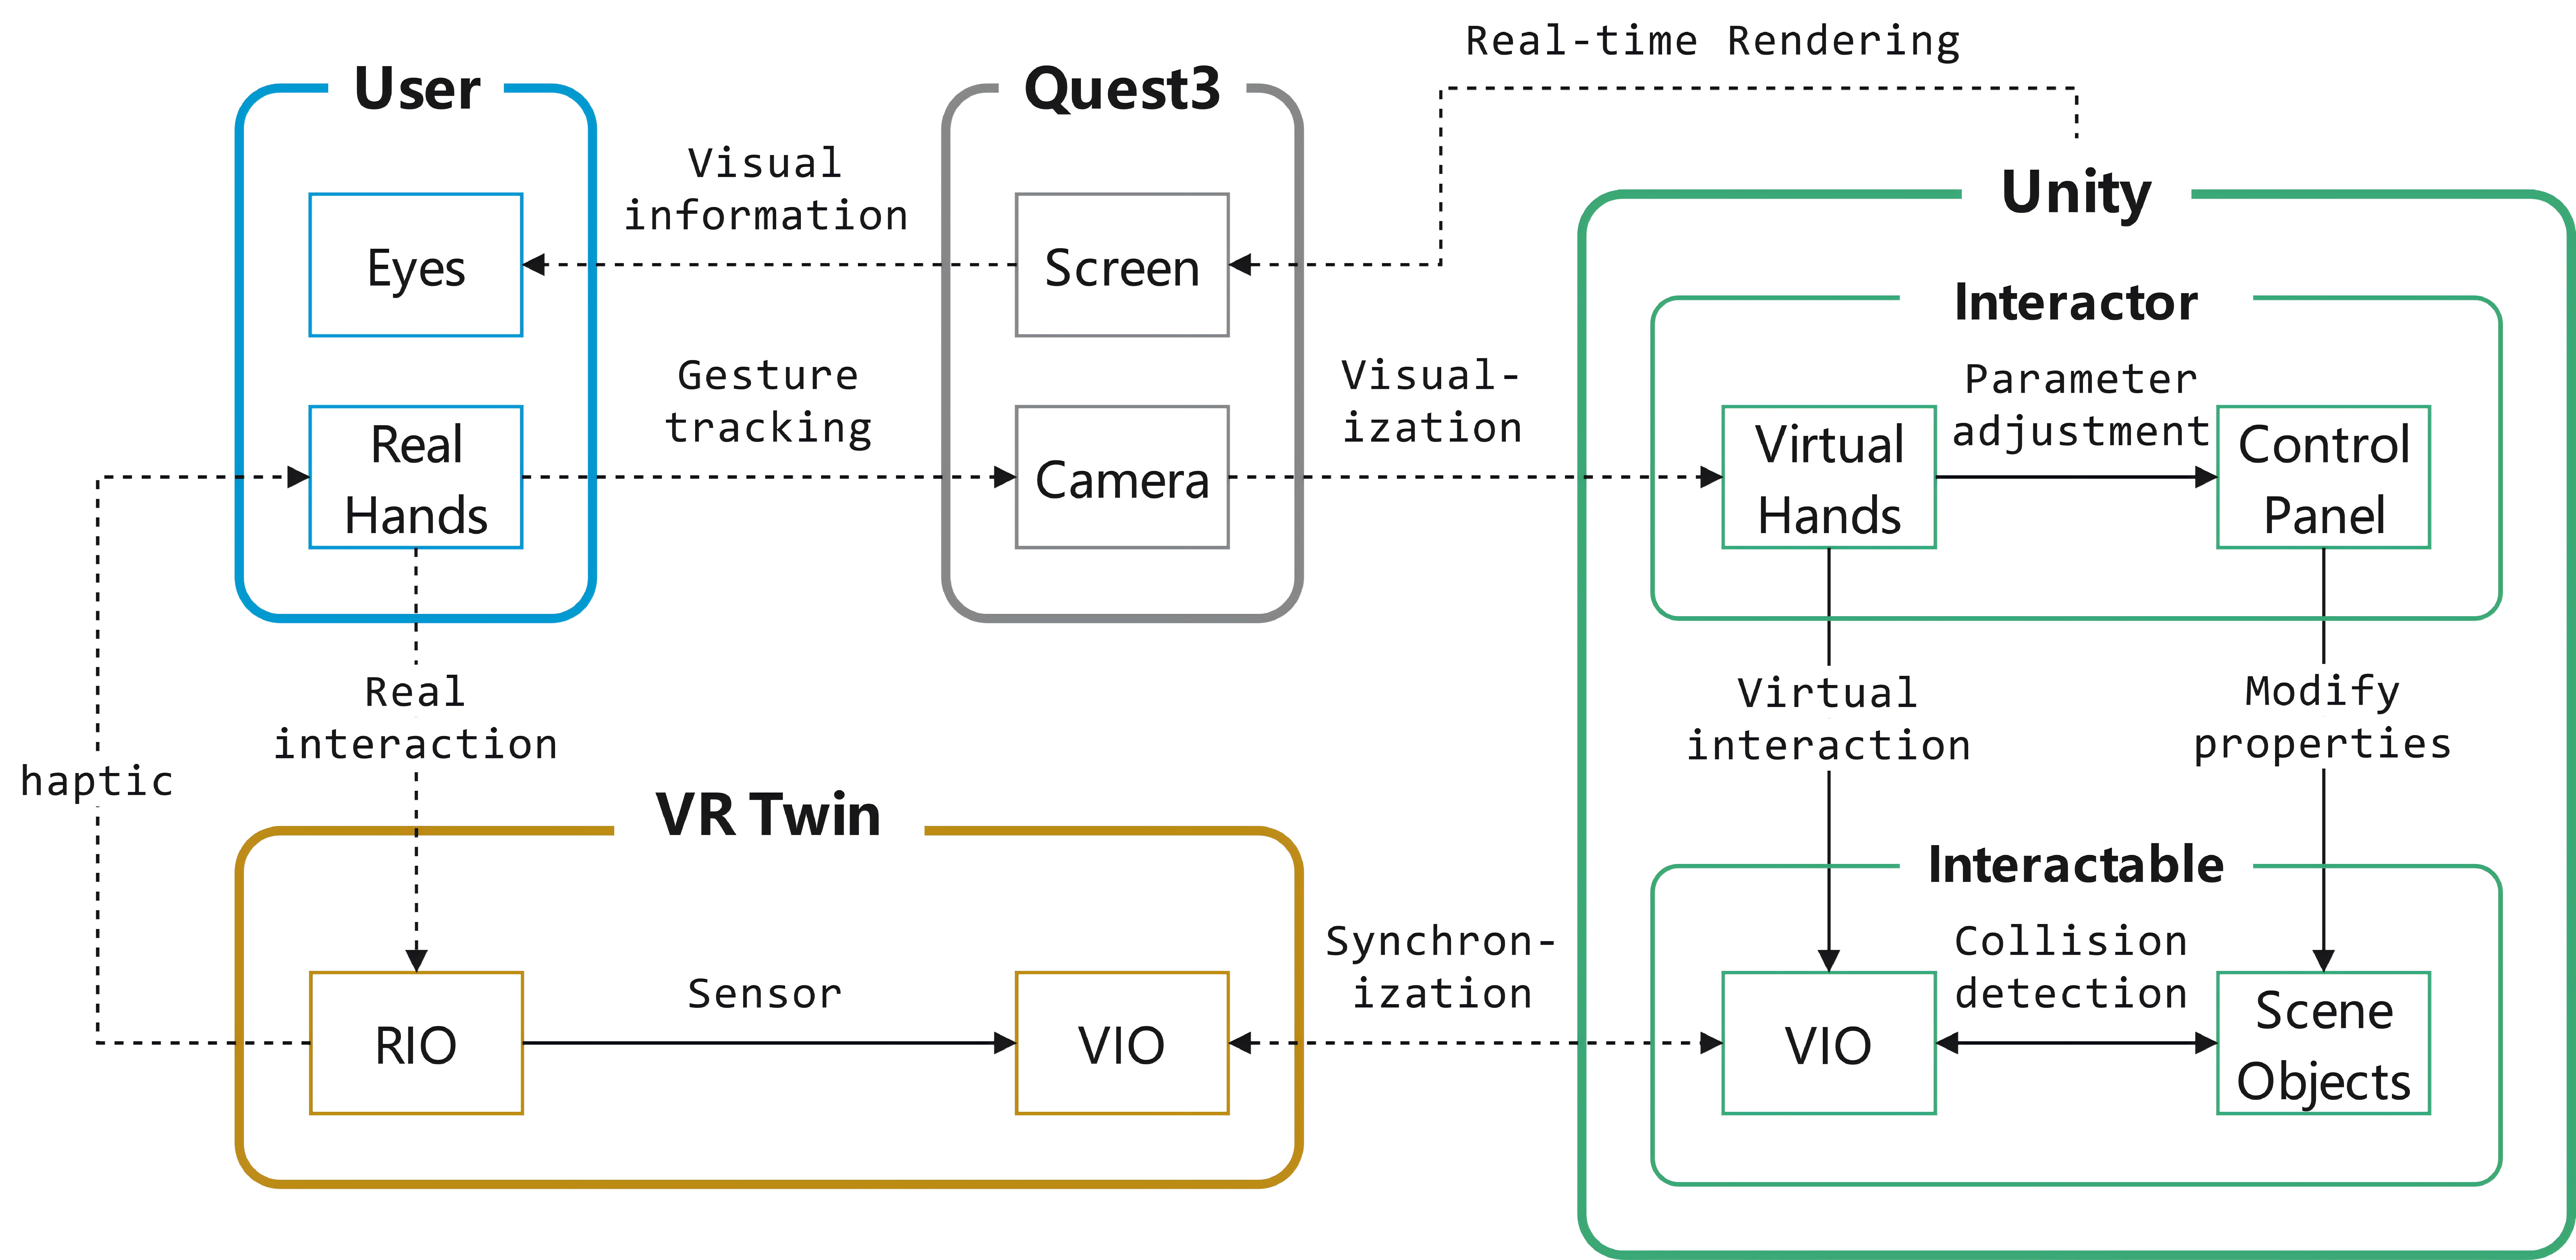
\includegraphics[width=1\textwidth]{image/system-framework-flowchart.pdf}
  \caption{系统框架流程图}
  \label{fig:system-framework-flowchart}
\end{figure*}

\subsection{评估方法}
本研究比较VRTI(具真实触觉反馈,实验组)和GI(无真实触觉反馈,对照组)。两种交互方式唯一区别在于是否具备真实触觉反馈。通过对照实验,探究真实触觉反馈对学生物理实验的认知负荷、学习动机、沉浸感和学习效果的影响。

\subsubsection{用户体验}
\begin{enumerate}
  \item {\texttt{认知负荷}}:采用Klepsch量表 \cite{klepsch2017development} 测量三个维度:内部认知负荷、外部认知负荷和关联认知负荷。触觉反馈任务中,触觉与视觉/听觉信息的多模态交互可能通过"注意力引导"降低外部认知负荷,但也可能因"跨模态切换"增加关联认知负荷
  \item {\texttt{学习动机}}:采用Keller量表 \cite{keller1983motivational},基于ARCS动机模型评估四个维度:注意力、相关性、信心和满意度,衡量学习者参与和完成学习任务的内驱力。接触触觉反馈等新技术时,学习者的内在动机(如好奇心和探索欲)或外在动机(如任务完成奖励)可能显著影响其参与度和学习效果。更高动机增加学生克服挑战的可能性,从而有效利用触觉反馈技术学习
  \item {\texttt{沉浸感}}:采用Schubert量表 \cite{schubert2001experience},聚焦虚拟环境中的临场感,通过空间临场感、参与度和虚拟环境真实感三个维度综合评估学生沉浸感和控制感
\end{enumerate}

所有量表均经翻译和本地化确保适合本实验文化和教育背景。

\subsubsection{物理知识}
物理知识测试由XXX大学物理系XXX教授团队提供,包含前测和后测:
\begin{enumerate}
  \item {\texttt{前测}}:含16题,其中6题聚焦基础物理知识评估学生基础理解,10题关联实验内容供与后测比较
  \item {\texttt{后测}}:含16题,其中10题与前测实验题相似(叙述和数据变化),6题难度更高的综合应用题评估学生批判性思维和知识整合能力
\end{enumerate}

两测试均含"我不知道"选项以减少猜测倾向,获取更准确评估数据。

\subsubsection{半结构化访谈}
用户实验后进行半结构化访谈探索参与者对VRTI和沉浸式学习的体验,通过追问深入探讨。例如:
\begin{enumerate}
  \item "您对VRTI的总体印象如何?"
  \item "您认为VRTI与GI的主要区别是什么?"
  \item "您提到'沉浸感',能否举例说明?"
\end{enumerate}
访谈旨在捕捉个性化观点和深度见解,同时确保数据完整性。在获得参与者同意后,在私密无干扰环境中进行面对面访谈,录音并记录笔记。

\subsection{评估流程}
\subsubsection{参与者}
招募XXX学校64名高中二年级学生参与实验。所有参与者均已在课堂学习相关基础物理知识。学生随机均分两组:
\begin{enumerate}
  \item 实验组(N=32):使用VRTI
  \item 对照组(N=32):使用GI
\end{enumerate}

\subsubsection{实验流程}
为确保结果有效性,所有参与者实验前接受统一实验介绍和操作指导(图\ref{fig:experimental-procedure})。流程含以下四步:
\begin{enumerate}
\item {\texttt{前测}}:学生独立完成前测问卷(约10分钟)
\item {\texttt{实验介绍}}:学生观看指导视频熟悉实验操作流程(约5分钟)
\item {\texttt{实验操作}}:学生按分组进行实验(约15分钟)
\item {\texttt{后测}}:学生独立完成后测问卷,含30项用户体验评估(认知负荷、学习动机、沉浸感)和15项物理知识评估(约30分钟)

\begin{figure}
  \begin{subfigure}{0.48\linewidth}
    \centering
    \includegraphics[width=\linewidth]{image/experimental-introduction.pdf}
    \caption{}
    \label{fig:experimental-introduction}
  \end{subfigure}
  \hfill
  \begin{subfigure}{0.48\linewidth}
    \centering
    \includegraphics[width=\linewidth]{image/experimental-operation.pdf}
    \caption{}
    \label{fig:experimental-operation}
  \end{subfigure}
  \caption{实验流程演示。(\subref{fig:experimental-introduction})实验介绍,(\subref{fig:experimental-operation})实验操作}
  \label{fig:experimental-procedure}
\end{figure}
\end{enumerate}

实验全程随机分配组别确保组间平衡,助教监督确保每位参与者严格遵循流程。

\subsection{结果分析}
\begin{figure*}[t]
  \centering
  \begin{subfigure}{0.45\textwidth}
    \centering
    \includegraphics[width=\linewidth]{image/pre-test-result.pdf}
    \caption{}
    \label{fig:pre-test-result}
  \end{subfigure}
  \hspace{0.05\textwidth}
  \begin{subfigure}{0.45\textwidth}
    \centering
    \includegraphics[width=\linewidth]{image/user-experience-result.pdf}
    \caption{}
    \label{fig:user-experience-result}
  \end{subfigure}
  \caption{前测与用户体验结果。(\subref{fig:pre-test-result})前测结果,(\subref{fig:user-experience-result})用户体验结果}
  \label{fig:pre-test-and-user-experience-result}
\end{figure*}

\begin{figure*}[t]
  \centering
  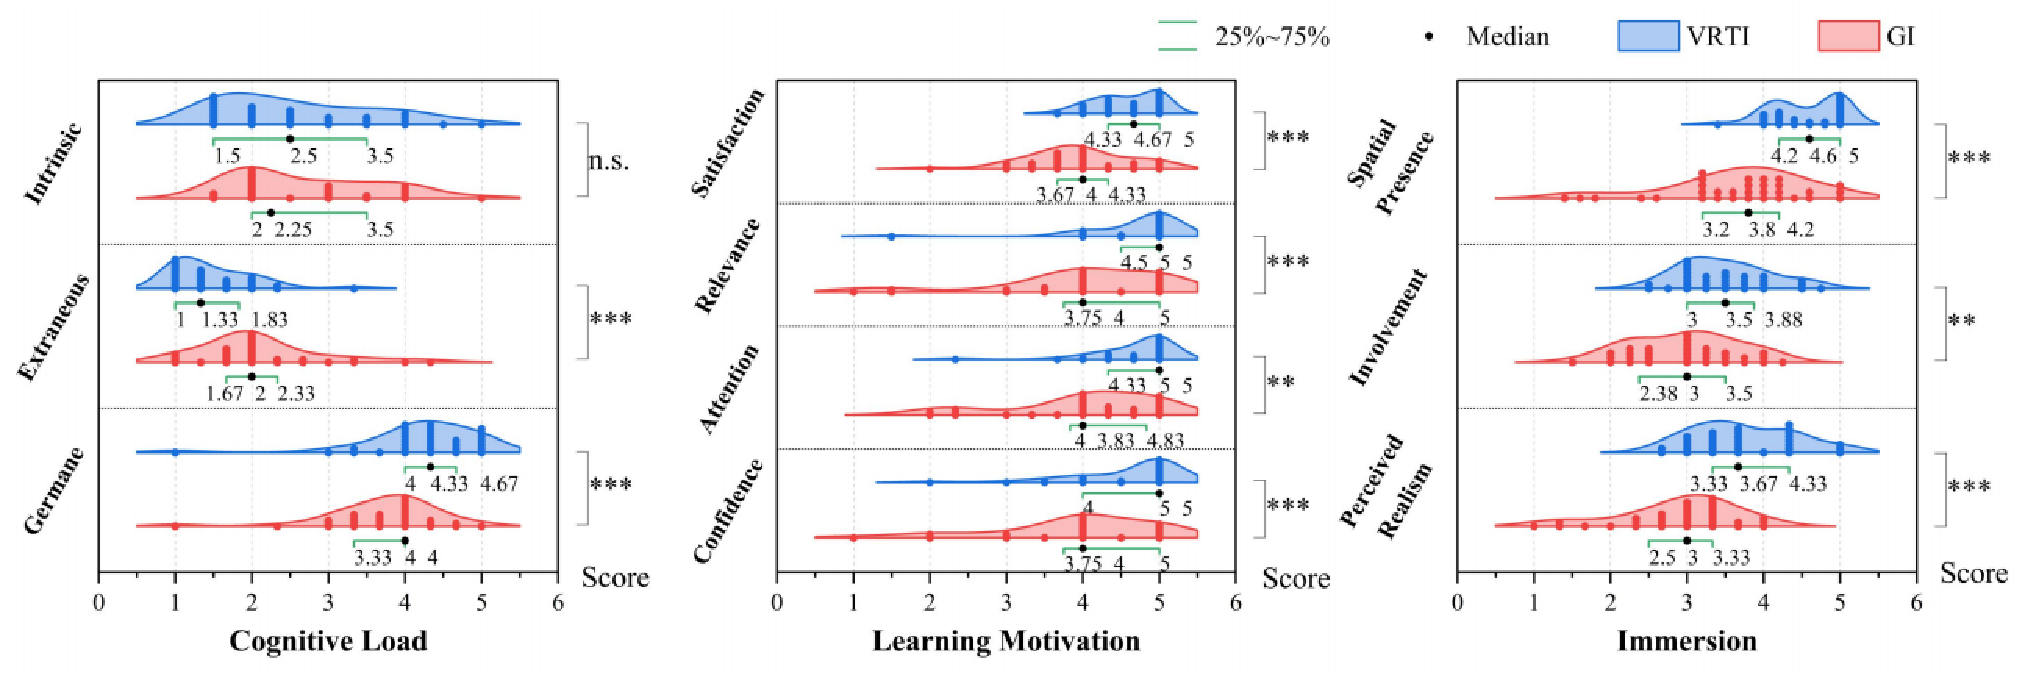
\includegraphics[width=\textwidth]{image/three-user-experience-result.pdf}
  \caption{VRTI与GI各用户体验维度对比}
  \label{fig:three-user-experience-result}
\end{figure*}

Shapiro-Wilks检验显示仅实验组实验相关内容测试结果服从正态分布,其余指标均违反该假设。故采用Mann-Whitney U检验分析组间差异。显著性水平:$p \le 0.05$ (*)表示显著差异,$p \le 0.01$ (**)表示高度显著差异,$p \le 0.001$ (***)表示极其显著差异。效应量解释:$|r| \le 0.1$为小效应,$0.1 < |r| \le  0.3$为中效应,$d > 0.5$为大效应。

\subsubsection{先验分析}
前测含6道基础物理概念题和10道实验相关题,每题1分共16分。图\ref{fig:pre-test-result}展示两组前测结果,柱长表示均值(Mean),黑色误差条表示1.0×标准差(SD)。Mann-Whitney U检验(M-U检验)显示实验组与对照组在基础物理概念($p=0.600$)、动量守恒知识($p=0.984$)和总分($p=0.834$)上均无显著差异。因此可认定两组具备相当的物理先验知识。

图\ref{fig:user-experience-result}对比实验组与对照组在认知负荷、学习动机和沉浸感三个维度的用户体验。各组上方实心圆点为样本点,核平滑拟合曲线描述其分布。下方I型箱线图展示25\%(Q1)、50\%(Q2)和75\%(Q3)分位数。

\subsubsection{认知负荷}
两组内部认知负荷无显著差异($Z=-0.720, p=0.472, |r|=0.127$)。实验组外部认知负荷显著低于对照组($Z=-3.538, p<0.001, |r|=0.625$),呈大效应量。相反,实验组关联认知负荷显著更高($Z=-3.337, p=0.001, |r|=0.590$),亦呈大效应量。可解释如下:
\begin{enumerate}
\item {\texttt{内部认知负荷}}:真实触觉反馈的加入不影响学习任务固有复杂性,符合认知负荷理论。内部认知负荷与任务本质复杂度相关,难以通过交互方式显著改变
\item {\texttt{外部认知负荷}}:VRTI通过提供真实触觉反馈,减少操作中冗余或干扰信息引起的不必要负荷
\item {\texttt{关联认知负荷}}:真实触觉反馈促进认知结构的构建和自动化,增强学习与理解
\end{enumerate}

\subsubsection{学习动机}
实验组在注意力($Z=-3.382, p=0.001, |r|=0.598$)、相关性($Z=-3.313, p=0.001, |r|=0.586$)、信心($Z=-3.001, p=0.003, |r|=0.531$)和满意度($Z=-4.127, p<0.001, |r|=0.730$)均显著提升,且均呈大效应量。可解释如下:
\begin{enumerate}
  \item {\texttt{注意力}}:沉浸式学习环境中的真实触觉反馈更有效吸引学习者兴趣
  \item {\texttt{相关性}}:定制化内容设计增强学习材料与学习者的关联性
  \item {\texttt{信心}}:VRTI提供的即时反馈和交互体验提升学习者信心
  \item {\texttt{满意度}}:真实触觉反馈在交互中提供成就感,增加学习者满意度
\end{enumerate}

\subsubsection{沉浸感}
实验组在空间临场感($Z=-4.524, p<0.001, |r|=0.800$)、参与度($Z=-2.774, p=0.006, |r|=0.490$)和真实感($Z=-4.102, p<0.001, |r|=0.725$)均显著提升,且呈大效应量。可解释如下:
\begin{enumerate}
  \item {\texttt{空间临场感}}:真实触觉反馈显著增强学习者的空间存在感
  \item {\texttt{参与度}}:VR孪生体的精心设计交互显著提升学习者投入度
  \item {\texttt{真实感}}:VRTI的高保真视觉与触觉体验显著提升学习环境真实感
\end{enumerate}

\subsubsection{学习效果}
图\ref{fig:improvements-result}展示动量概念、实验理解和总分的前后测提升比较结果,以及综合应用表现。动量概念和实验理解评估各含5题,每题1分(共10分)。

实验组在实验理解方面提升显著($Z=-1.967, p=0.05, |r|=0.347$),呈中效应量;但在动量概念($Z=-0.354, p=0.724, |r|=0.063$)和总分($Z=-1.714, p=0.087, |r|=0.303$)上无显著提升。此外,实验组在综合应用测试中表现显著更好($Z=-2.828, p=0.005, |r|=0.500$),呈大效应量。这表明VRTI通过真实触觉反馈帮助学习者更直观理解实验内容,并提升综合应用能力。但动量概念的掌握更依赖学习者先验知识和抽象思维能力,VRTI影响有限。

\begin{figure}
  \centering
  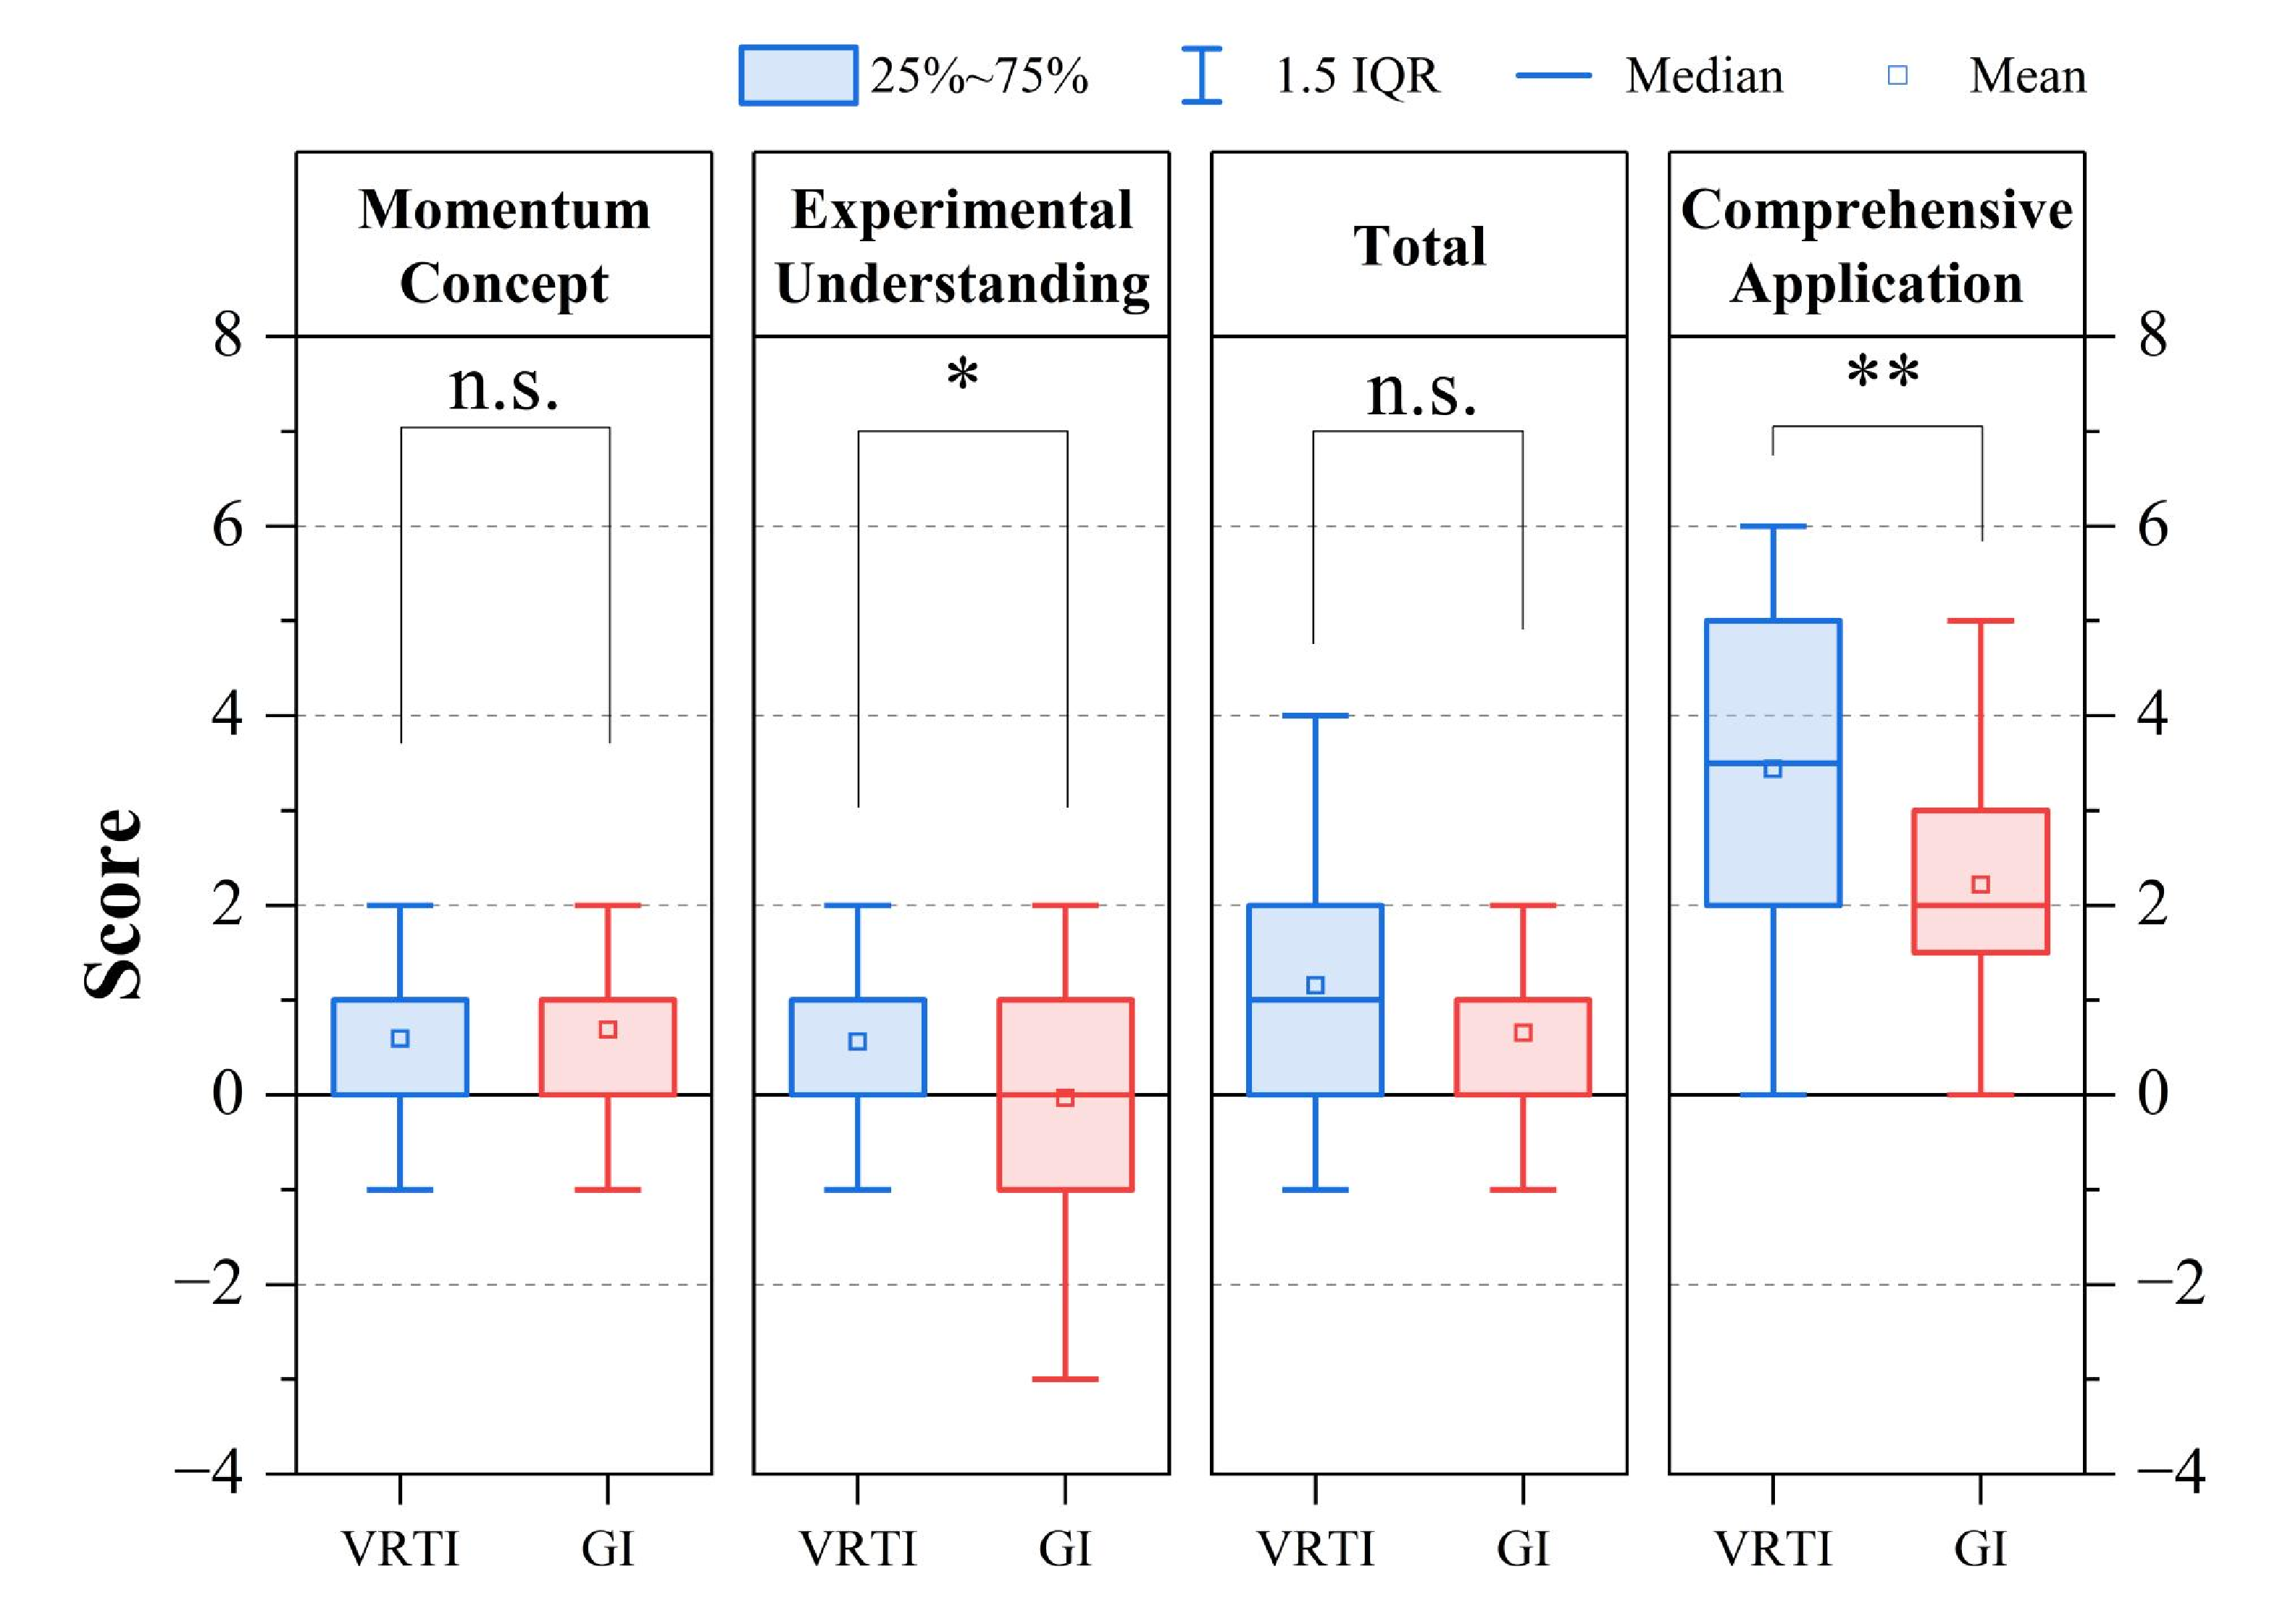
\includegraphics[width=0.8\linewidth]{image/improvements-result.pdf}
  \caption{动量概念、实验理解和总分的前后测提升及综合应用表现对比结果}
  \label{fig:improvements-result}
\end{figure}

\subsubsection{访谈结果}
实验后对参与者进行半结构化访谈,探究其对VRTI和GI的主观体验。主要发现包括:
\begin{enumerate}
  \item {\texttt{整体体验}}:多数用户对触觉反馈给予积极评价,一名用户表示:"VRTI让我感受到物体的重量和阻力,操作更具沉浸感"。但有用户提到长时间使用GI会导致手臂疲劳:"GI中手臂长时间悬空让我感到疲惫"
  \item {\texttt{与GI对比}}:用户普遍认为VRTI在触觉反馈和操作直观性上优于GI。一名用户指出:"GI提供运动自由度,但缺乏真实触觉反馈使其体验不完整"。相反,部分用户强调GI的灵活性:"GI允许自由调整手部位置,而VRTI需固定位置"
  \item {\texttt{沉浸体验}}:用户广泛认可VRTI显著增强其在虚拟环境中的沉浸感。一名用户解释:"当我拉动弹簧时能感受到阻力,仿佛在进行真实物理实验"。但有用户报告频繁使用后触觉反馈质量下降:"多次实验后设备触觉反馈响应性降低"
  \item {\texttt{改进建议}}:用户提出多项VRTI优化建议。例如建议优化设备支撑结构减少操作疲劳:"若设计支架避免手臂持续悬空,操作会更舒适"。此外用户强调需提升设备耐久性:"设备触觉反馈在重复使用后减弱,希望未来改进"
\end{enumerate}

\section{局限性与未来工作}
当前VR孪生系统中RIO和VIO的部署仍属半自动化,需手动调整确保精确对齐。本研究期间VR头显功能限制导致难以捕捉摄像头图像实现自动定位。仅依赖传感技术精确定位成本高昂且可能引入额外基站部署,增加系统复杂性。未来研究将探索全自动部署方法,使用户佩戴VR头显后即刻实现RIO精确定位和VIO实时重建。通过集成先进计算机视觉技术和机器学习算法,实现对齐误差的动态预测与调整,达成无需人工干预的空间对齐。

另一局限是当前系统仅支持单用户交互,而多用户场景(如小组实验或团队问题解决活动)需同步交互和共享虚拟环境。未来研究将探索多用户交互扩展,重点开发支持协作活动的共享虚拟环境。此外将探究VRTI的教育价值,特别是在VR协作学习模式中的应用。

用户反馈还凸显触觉反馈设备耐久性和长时间交互的身体疲劳问题,可能影响系统长期可用性和用户满意度。未来研究将优先提升交互设备耐久性,采用先进材料改善触觉反馈设备寿命和响应性,同时融入人机工学设计原则减少用户交互负担。

最后,当前系统的实验设置和用户交互依赖预定义规则,限制了其对多样化学习场景和个性化学习需求的适应性。未来研究将聚焦AI与VRTI的集成,分析用户行为、预测学习需求并动态调整实验环境。例如AI可引导用户完成复杂实验,提供个性化反馈并根据进度推荐补充学习资源。AI驱动的数据分析还可评估学习效果,为系统和课程改进提供依据。

\section{结论}
本文针对VR沉浸式学习环境中手势交互(GI)缺乏触觉反馈的问题,提出虚拟-现实孪生交互(VRTI)。针对高中物理学习中的动量守恒实验,设计实现支持抓握、按压和捏取操作的三种虚拟-现实孪生体(VR孪生体)。在动量守恒实验场景中对比评估VRTI与GI表明,前者显著提升用户学习动机和沉浸感且未显著增加认知负荷,同时更好帮助用户理解实验内容并提升知识综合应用能力。未来研究将探索VR孪生体在其他物理学习场景的应用,改进硬件结构并优化交互方式以提升用户学习体验和操作舒适度。

\begin{credits}
\subsubsection{\ackname} 
本研究得到国家自然科学基金(编号62377004)支持。

\subsubsection{\discintname}
作者声明无利益冲突。
\end{credits}

% \setlistofchangestitle{修订历史}
% \listofchanges

\bibliography{VRTI-bib}

\end{document}